\section{Система інтелектуальної власності}\marginpar{\framebox{01.09.2015}}
\subsection{Основні поняття та визначення}
\textbf{Право ІВ} - це право на результат творчої діяльності людини.

\textbf{ОПІВ} - об’єкт права інтелектуальної власності. \textbf{Завжди} нематеріальний.

Право ІВ має подвійну природу: 
\begin{itemize}
	\item Особисте немайнове право
	\item Майнове право
\end{itemize}

Особисте немайнове право невіддільне від автора і немає обмежень у просторі та часі. Складається з
\begin{itemize}
	\item Право людини на визнання її творцем ОПІВ
	\item Право на перешкоджання такого використання ОПІВ, яке може завдати шкоди честі чи репутації автора
	\item Інші особисті немайнові права передбачені законодавством (право оприлюднювати твір анонімно, під псевдонімом і так далі)
\end{itemize}

Майнові права віддільні від автора і мають обмеження у просторі та часі. Складаються з
\begin{itemize}
	\item Право використовувати ОПІВ у власній господарській діяльності
	\item Виключне право дозволяти використання ОПІВ іншим особам
	\item Виключне право перешкоджати неправомірному використанню ОПІВ
	\item Інші майнові права передбачені законодавством
\end{itemize}

Право на ОПІВ і право на матеріальний об’єкт в якому цей ОПІВ втілено незалежні одне від одного. 

В загальному розумінні право ІВ тримається на трьох моментах:
\begin{itemize}
	\item Авторство (хто автор)
	\item Пріоритет (хто перший)
	\item Обсяг охорони (що ми охороняємо)
\end{itemize}
\subsection{Класифікація ОПІВ}
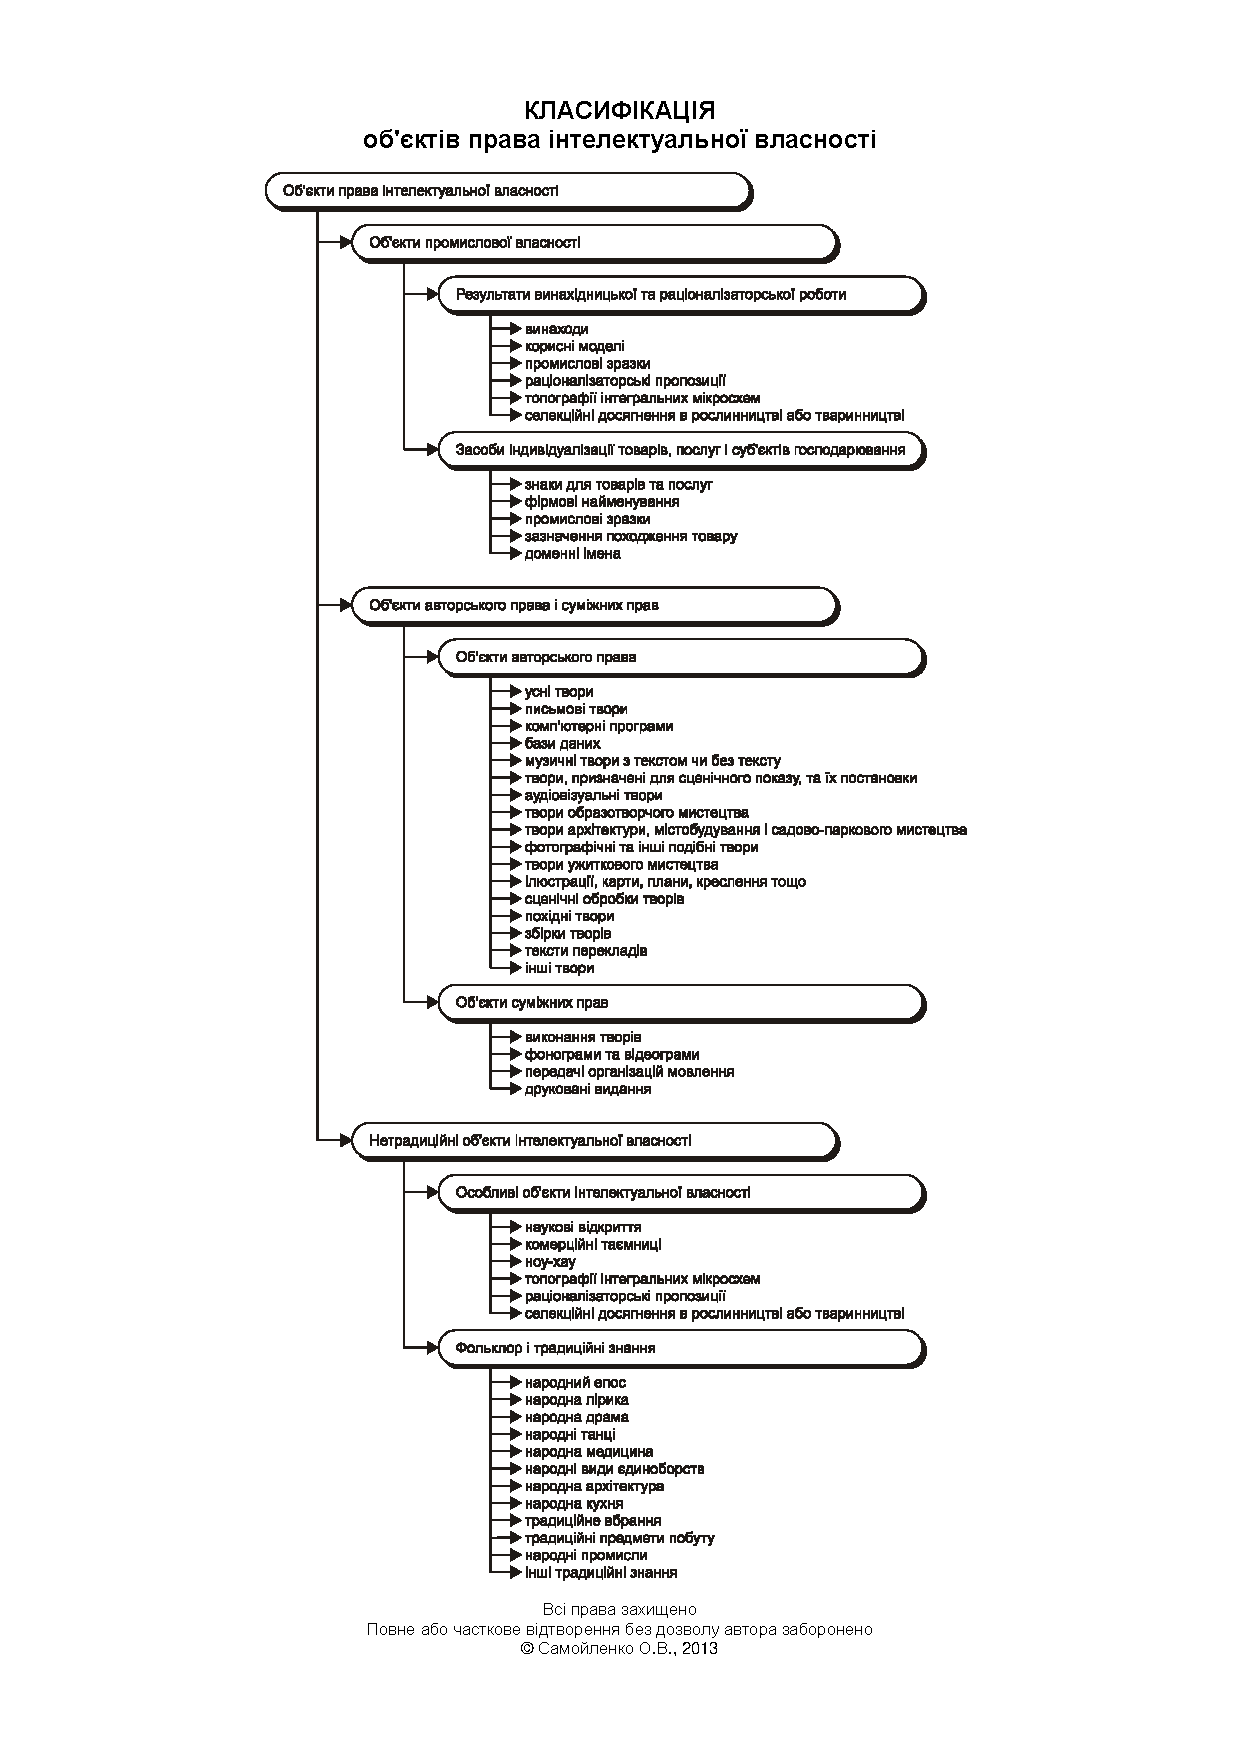
\includegraphics[scale=0.75]{opiv.pdf}
Об’єкти промислової власності названі так тому, що використовуються в основному у промисловості. Не плутати з промисловими потужностями. Головною особливістю ОПВ (об’єктів промислової власності) є те, що права на них виникають після успішного проходження ряду експертиз та виконання інших обов’язкових формальностей. 

Об’єкт суміжного права та суміжних прав. Відрізняється від ОПВ тим, що права на них виникають автоматично за фактом створення твору. І для виникнення прав не обхідно жодних формальностей.
